\documentclass[11pt]{article}
\usepackage{charter}
\usepackage{graphicx}
\usepackage{hyperref}
\usepackage{mdframed}
\usepackage[margin=1in]{geometry}
\usepackage{amsmath,amssymb}

\hypersetup{
	colorlinks=true,
	linkcolor=blue,
	filecolor=magenta,
	urlcolor=cyan,
}

\begin{document}

%===================================================
% Title and Author Info
%===================================================
\begin{center}
{\Large\textsc{Relativistic Orbits}} \\
\vspace{10pt}
{\large \textbf{Mentor:} Alex Urban} \\
{\small LIGO Laboratory, California Institute of Technology \\
Pasadena, CA 91125, USA \\
\href{mailto:aurban@ligo.caltech.edu}{\texttt{aurban@ligo.caltech.edu}}}
\end{center}

%%%%%%%%%%%%%%%%%%%%%%%%%%%%%%%%%%%%%%%%%%%%%%%%%%%

\section*{Orbital Death Spirals and Hydrostatic Equilibrium}
\hspace{15pt} Suppose that a compact binary with masses $m_1$, $m_2$ is in a stable circular orbit. This time, we'll model its energy loss due to gravitational waves. Figure \ref{fig:binary_diagram} illustrates this system.

\vspace{20pt}

\begin{figure}[!h]
\begin{mdframed}
\centering
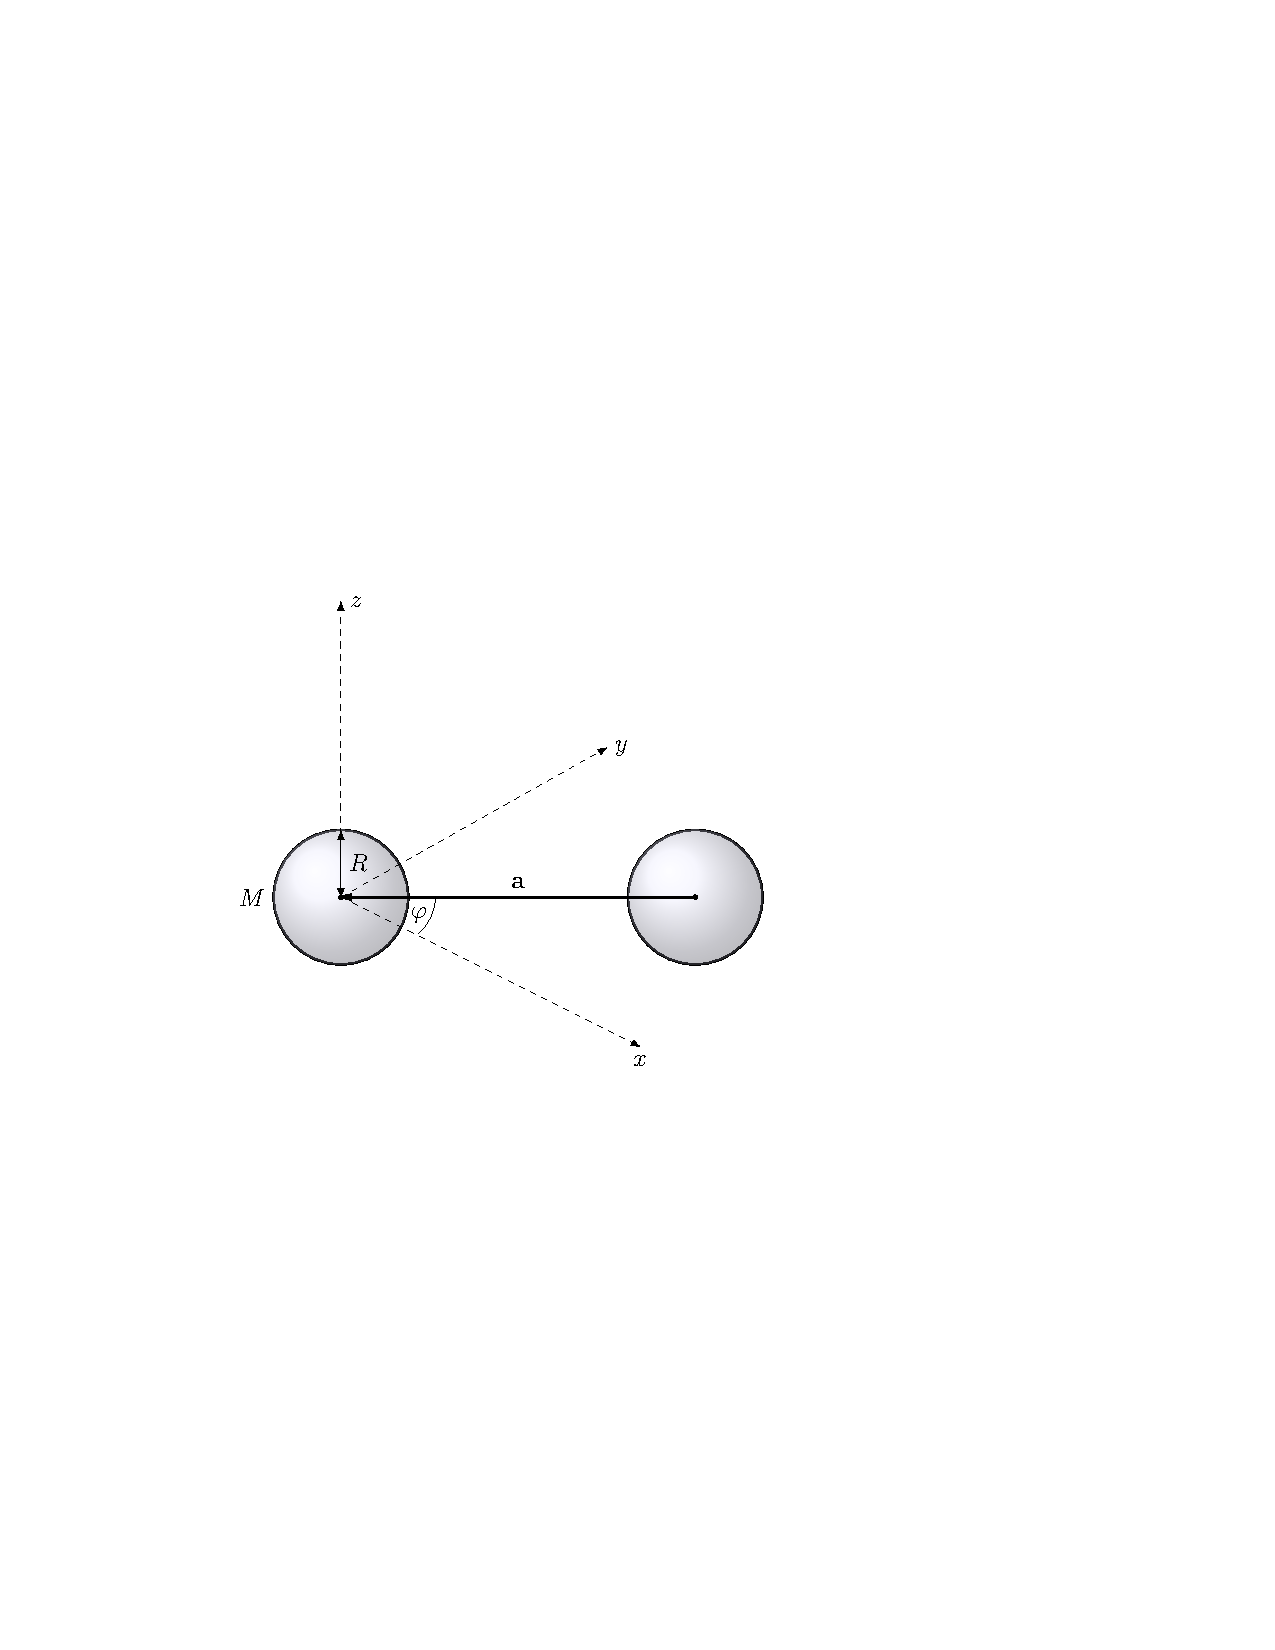
\includegraphics{relativistic_orbit/binary_diagram.pdf}
\caption{\label{fig:binary_diagram}Diagram of the neutron star binary in the center of mass frame, showing its orbital separation vector ($\mathbf{r}$) and the radius ($R$) and masses ($m_1$, $m_2$) of the individual neutron stars. The azimuthal angle $\varphi$ is also indicated.}
\end{mdframed}
\end{figure}

\vspace{10pt}

As we have seen, the orbiting binary is a simple example of a system with nonzero \textit{quadrupole moment} that changes over time. According to general relativity, this means the system will emit gravitational waves, which carry orbital energy away at a rate
\begin{equation}\label{eq:GW_luminosity}
L_{\rm GW} = \frac{dE}{dt} = - \frac{32}{5} \frac{G^4}{c^5} \frac{\mu^2 M^3}{r^5}
\end{equation}
where $M = m_1 + m_2$ is the total mass and $\mu = m_1 m_2/(m_1 + m_2)$ is the reduced mass. (This is the observed ``luminosity'' in gravitational waves, which are emitted at twice the orbital frequency.)

\vspace{1000pt}

\begin{enumerate}

\item Using the fact that the gravitational binding energy of this system at a given time is
\[ E = - \frac{GM\mu}{2r}, \]
show that the orbital separation $r$ varies like
\begin{equation}\label{eq:drdt}
\frac{dr}{dt} = - \frac{64}{5} \frac{G^3}{c^5} \frac{\mu M^2}{r^3}.
\end{equation}
Can you solve this equation the old-fashioned way (\textit{i.e.} with pen and paper)?

\item How long does it take the orbit to evolve from a gravitational wave frequency of 20 Hz up to the ISCO frequency? Express this in terms of $\mu$ and $M$.

\item Numerically integrate equations \ref{eq:GW_luminosity} and \ref{eq:drdt} for a neutron star system with $m_1 = m_2 =$ 1.4 $M_{\odot}$. Plot the orbital separation, orbital velocity ($v/c$), kinetic, potential, and total energies, GW frequency, and the GW luminosity, all as a function of time. (You can start the integration from a separation of 500 km, and follow it all the way up to ISCO. Use the Schwarzschild potential we've been exploring for the past couple of weeks.)

\item Now, let's switch gears a bit and start building a model of very dense stellar material. To begin with, use Newtonian physics to try and show that an outward pressure on a spherical star will balance the inward pull of the star's gravity exactly when
\begin{equation}\label{eq:hydro}
\frac{dP}{dr} = - \frac{G}{r^2}\, \rho(r)\, m(r),
\end{equation}
where $\rho(r)$ is called the \textit{density profile} and
\begin{equation}\label{eq:mass}
\frac{dm}{dr} = 4 \pi r^2 \rho(r)
\end{equation}
is the mass contained in a shell of radius $r$. (This condition, and the physical state it describes, is called \textit{hydrostatic equilibrium}.) What do $P(r)$ and $m(r)$ look like when the star is uniformly dense (so $\rho$ is a constant)?

\item In astrophysics, a \textit{polytrope} loosely refers to any object whose internal pressure and density are related by
\begin{equation}\label{eq:polytrope}
P = K \rho^{\gamma}
\end{equation}
where $K$ and $\gamma$ are constants. In particular, we can imagine, say, a gas of electrons that produce an outward pressure because no two of them can ever occupy the same quantum state (the Pauli exclusion principle). In this case, $\gamma =$ 5/3 and
\[ K = \frac{\hslash^2}{15\pi^2 m_e} \left( \frac{3\pi^2}{n m_N} \right)^{5/3} \]
where $m_e$ is the electron mass, $m_N$ the neutron mass, and $n$ the number of nucleons per electron. Try solving Eqs. \ref{eq:hydro} and \ref{eq:mass} numerically using this equation of state with $n=2$, which is a good model for a white dwarf star of total mass 1 $M_{\odot}$ and radius 10$^4$ km that's made mostly of neutral carbon.

\end{enumerate}

%%%%%%%%%%%%%%%%%%%%%%%%%%%%%%%%%%%%%%%%%%%%%%%%%%%

\section*{Things That Make You Go, ``Hmmm....''}

\begin{enumerate}

\item How does the rate of orbital decay (Eq. \ref{eq:drdt}) compare with the orbital velocity during your model of an inspiral?

\item Can you use this to justify the approximation we talked about last time, in which we can ignore radial acceleration when we account for forces during the inspiral?

\item What physics is the Newtonian condition for hydrostatic equilibrium (Eq. \ref{eq:hydro}) failing to capture?

\end{enumerate}

\end{document}
